\chapter{Image Data Transformation}

We can attempt to classify the raw image data; the image being represented as a vector of light intensities at each pixel. However, it might be beneficial to transform the image data into a feature space using a feature extraction technique. The feature extraction techniques can be split into two categories. Local feature extractors and global feature extractors. %https://link.springer.com/content/pdf/10.1007%2F978-3-540-31638-1.pdf 219-

Local feature extractors localise such points in an image, which could be found regardless of the image subject position. These points are called key-points. The area around such key-points is then described using a vector called descriptor. The descriptors are created in a way, which allows for matching similar features.

Global feature extractors transform the whole image into a lower dimensional vector, attempting to retain the most important information.

For feature extraction, we compare three local feature extractors: SIFT, SURF and ORB and a global feature extractor: PCA.

In this section, we describe the four feature extraction algorithms.

\section{SIFT}
SIFT (Scale Invariant Feature Transform) was  proposed by David Lowe, and published in the original paper \cite{Lowe1999} in 1999. SIFT.

Compared to ordinary techniques such as the Harris Corner Detector \cite{Harris1988} or Canny edge detector \cite{Canny1986}, the SIFT identifies the general (not only edges and corners) key-points. The descriptors, which describe the local image region around the key-points are scale invariant. Moreover, they are invariant to rotation, illumination and to change in affine transformations. In our text, we introduce the methodology of training the classifier that recognizes the objects in real images (photographs); therefore the properties of SIFT feature vector are essential.

\subsection{Key-point Detection}

Let us consider an input image \( I_{img}(x,y) \). A convolution of the image with a Gaussian kernel
\begin{equation}
    G(x,y,\sigma) = \frac{1}{2\pi\sigma^2}e^{-\frac{x^2+y^2}{2\sigma^2}},
    \label{eq:Gaussian_kernel}
\end{equation}
at a scale \( \sigma \) is exploited to get a scale-space representation of the image, so that:
\begin{equation}
    L(x, y,\sigma) =  G(x,y,\sigma)*I_{img}(x,y).
\end{equation}

In order to detect scale invariant key-points, scale normalised Laplacian of Gaussian (LoG)
\begin{equation}
    \Laplace_{norm} L(x, y, \sigma) = \sigma\left(\frac{\partial^2 L(x,y,\sigma)}{\partial x^2} + \frac{\partial^2 L(x,y,\sigma)}{\partial y^2}\right)
\end{equation}
is required \cite{Koenderink1984}. It has been shown \cite{Mikolajczyk2002}, that local extrema of LoG provide the most stable image features, compared to many other popular image functions.

Determination of the LoG would be time consuming, therefore, it is approximated by the Difference of Gaussian (DoG)\cite{Lowe2004}.The DoG is computed from two adjacent scales separated by a constant multiplicative factor $k \in \mathbb{R}$:
\begin{equation}
    D(x,y,\sigma) := L(x,y,k\sigma) - L(x,y,\sigma).
\end{equation}

To ensure scale invariance, the extrema are located not only in the domain of one DoG, however it is found across different scales as well. The different DoGs at the scales are created by progressively convolving the original image with the Gaussian kernel. The consecutive Gaussian kernels' scale differs by the multiplicative factor $k$.

At each doubling of the scale $k$, the resolution of an image can be reduced by factor of $2$ for efficiency. Each group of blurred images of the same resolution is called an octave. In each octave, we generate the DoG by subtracting the $L(x, y, \sigma)$ of neighbouring scales. This is called the DoG pyramid and can be seen in \figref{fig:DoG_pyramid}.

\begin{figure}
    \centering
    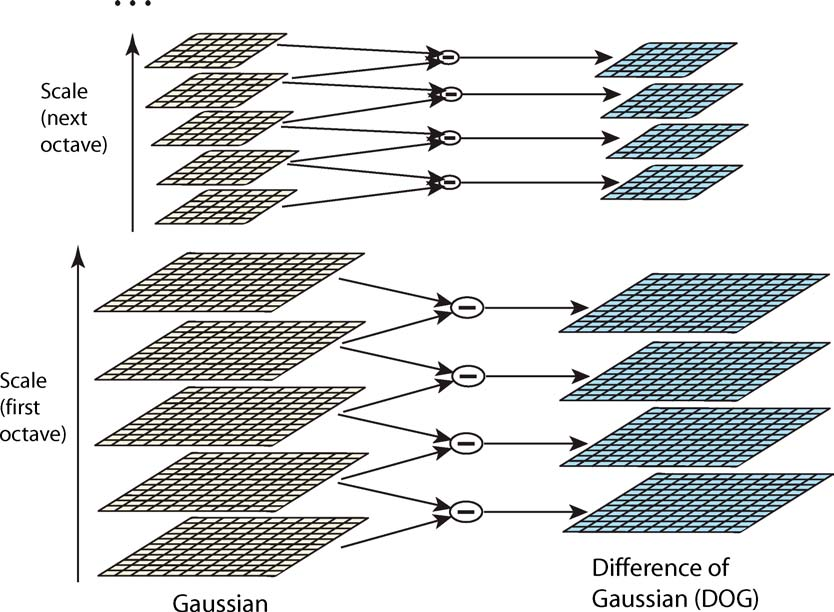
\includegraphics[width=0.8\textwidth]{Figures/sift/pyramid.jpg}
    \caption[DoG pyramid.]{DoG pyramid. \cite{Lowe2004}}
    \label{fig:DoG_pyramid}
\end{figure}

Each pixel in the DoG pyramid is compared to the $3\times3$ pixels in DoGs below and above, and to the $8$ surrounding pixels. This is shown in \figref{fig:DoG_extrema}. The pixel is selected as a key-point candidate, if it has lower or higher value than all of these $26$ pixels.

\begin{figure}
    \centering
    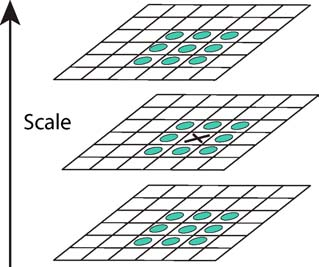
\includegraphics[width=0.4\textwidth]{Figures/sift/extrema.jpg}
    \caption[Optima of the DoG are selected by the means of comparing pixel to the 26 pixels surrounding it in the scale-space.]{Optima of the DoG are selected by the means of comparing pixel to the 26 pixels surrounding it in the scale-space. \cite{Lowe2004}}
    \label{fig:DoG_extrema}
\end{figure}

To detect a sub-pixel locations of extrema, the DoG is interpolated using quadratic Taylor expansion at each key-point candidate:
\begin{equation}
    D(\boldsymbol{x}) = D + \frac{\partial D^T}{\partial \boldsymbol{x}}\boldsymbol{x}+\frac{1}{2}\boldsymbol{x}^T\frac{\partial^2 D}{\partial \boldsymbol{x}^2}\boldsymbol{x},
    \label{eq:taylor_expansion}
\end{equation}
where \( D(x,y,\sigma) \) and the partial derivatives are evaluated at the key-point and \( \boldsymbol{x}=(x,y,\sigma) \) is the offset from the key-point. Then, extrema \( \hat{\boldsymbol{x}} \) is located by setting the gradient of \( D \) to be zero vector:
\begin{equation}
    \hat{\boldsymbol{x}} = - \frac{\partial^2 D^{-1}}{\partial \boldsymbol{x}^2}\frac{\partial D}{\partial \boldsymbol{x}}.
    \label{eq:taylor_extremum}
\end{equation}
If the offset \( \hat{\boldsymbol{x}} \) is larger than \( 0.5 \) in any dimension, it indicates that the extrema is closer to another point. In this case, the candidate point is changed to the new point and interpolation is performed again.

The function value at the sub-pixel extrema ,$D(\hat{\boldsymbol{x}})$, is used for rejecting extrema with low contrast. In our experiments, we use the OpenCV SIFT implementation default value $\frac{0.04}{3}$\cite{openCV}.

The DoG has a strong response along edges, even if the location along the edge is poorly determined. These candidate key-points have principal curvature perpendicular to the edge much larger than the principal curvature along it. The principal curvatures can be computed from a $2\times2$ Hessian matrix at the location of the key-point candidate
\begin{equation}
    \boldsymbol{H} =
    \begin{bmatrix}
        D_{xx} & D_{xy}\\
        D_{xy} & D_{yy}
    \end{bmatrix},
    \label{eq:hessian}
\end{equation}
where the partial derivatives are estimated by taking the differences of neighboring sample points. The eigenvalues of $\boldsymbol{H}$ are proportional to the principal curvatures.

The computation of eigenvalues can be avoided, as only the ratio of the eigenvalues is required. Let us denote the larger eigenvalue as $\alpha$ and the smaller one as $\beta$. The trace of $\boldsymbol{H}$ is defined as
\begin{equation}
    Tr(\boldsymbol{H}) = D_{xx}+D_{yy} = \alpha+\beta,
\end{equation}
and the determinant as
\begin{equation}
    Det(\boldsymbol{H}) = D_{xx}D_{yy}-D_{xy}^2 = \alpha\beta.
\end{equation}

Let $r$ be the ratio of the eigenvalues, such that
\begin{equation}
    r=\frac{\alpha}{\beta}.
\end{equation}
Then,
\begin{equation}
    \frac{Tr(H)^2}{Det(\boldsymbol{H})} = \frac{(\alpha+\beta)^2}{\alpha\beta}=\frac{(r\beta+\beta)^2}{r\beta^2} = \frac{(r+1)^2}{r}.
\end{equation}

Therefore, to inspect the ratio of eigenvalues, we can check
\begin{equation}
    \frac{Tr(H)^2}{Det(\boldsymbol{H})} = \frac{(\alpha+\beta)^2}{\alpha\beta}=\frac{(r\beta+\beta)^2}{r\beta^2} = \frac{(r+1)^2}{r}.
\end{equation}
The candidate key-points with this ratio below a threshold $r$ is discarded. In our experiments, we use the default value of OpenCV SIFT implementation: $10$.

\subsection{Key-point Description}
We want to create a descriptor for each of our key-points. These descriptors must be almost identical across different scale, rotation, illumination and other transformations.

In order to ensure descriptor invariance to a rotation, we first determine the key-point orientation. First, we calculate the gradient magnitude
\begin{equation}
    m(x,y) = \sqrt{(L(x+1,y)-L(x-1,y))^2+(L(x,y+1)-L(x,y-1))^2},
\end{equation}
and orientation
\begin{equation}
    \theta(x,y) = tan^{-1}\left(\frac{L(x,y+1)-L(x,y-1)}{L(x+1,y)-L(x-1,y)}\right),
\end{equation}
of each point within a region around the key-point. From these, an orientation histogram with $36$ bins is created. The largest peak is selected as a key-point orientation. If there are other peaks more than $80\%$ of the largest peak, new key-points are created at the same location with the other peaks as their orientation.

For the descriptor, a window $16\times16$ pixels around the key-point, rotated by the orientation of the key-point, is used. In this window, the gradient magnitude and the orientation is computed for each point. The $16\times16$ window is divided into $16$ ($4\times4$) sub-windows. For each sub-window, an $8$ bin gradient orientation histogram, weighted by gradient magnitudes, is created. This can be seen for smaller $8\times8$ window in \figref{fig:sift_descriptor}. These histograms then form a descriptor vector.

\begin{figure}
    \centering
    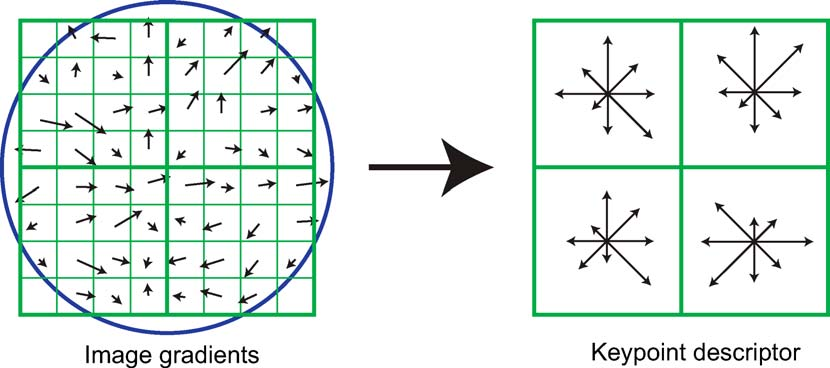
\includegraphics[width=0.8\textwidth]{Figures/sift/descriptor.jpg}
    \caption[Extracting the sift-descriptor.]{Building of the sift-descriptor. \cite{Lowe2004}}
    \label{fig:sift_descriptor}
\end{figure}


\section{Speeded Up Robust Features}
Speeded Up Robust Features (SURF) is a local feature transformation algorithm proposed by Herbert Bay, Tinne Tuytelaars, and Luc Van Gool in 2006 \cite{Bay2006}. Compared to SIFT \cite{Lowe1999}, the authors claim the SURF detector and descriptor to be faster and more robust against various image transformations.

\subsection{Key-point Detection}
The SURF key-point detection is based on the determinant of the Hessian matrix. Let us consider an input image $I_{img}(x,y)$ and the scale-space representation of the image
\begin{equation}
    L(x, y,\sigma) =  G(x,y,\sigma)*I_{img}(x,y),
\end{equation}
where $G(x,y,\sigma)$ is the Gaussian kernel defined in \eqref{eq:Gaussian_kernel}.

The Hessian matrix at scale $\sigma$ is defined as
\begin{equation}
    \mathcal{H}(x, y, \sigma) =
    \begin{bmatrix}
        L_{xx}(x, y, \sigma) & L_{xy}(x, y, \sigma)\\
        L_{xy}(x, y, \sigma) & L_{yy}(x, y, \sigma)
    \end{bmatrix},
\end{equation}
where $L_{xx}(x, y, \sigma)$, $L_{xy}(x, y, \sigma)$, and $L_{yy}(x, y, \sigma)$ are the second-order derivatives of the scale-space representation of the image at a point $(x, y)$.

The SURF authors decided to approximate the second order derivatives of Gaussian filter with box filters (shown in \figref{fig:Gauss_box_y}). Because the property of Gaussian filter, that no new structures can appear while going to a lower resolution, has been shown not to apply in 2D case \cite{Koenderink1984}, this can be done. Box filters allow for the use of integral images, which reduces the computational complexity.

\begin{figure}
    \centering
    \begin{subfigure}{0.24\textwidth}
        \centering
        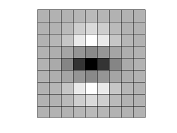
\includegraphics[width=\textwidth]{Figures/surf/y_gauss.png}
        \label{fig:y_gauss}
    \end{subfigure}
    \begin{subfigure}{0.24\textwidth}
        \centering
        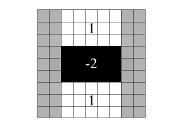
\includegraphics[width=\textwidth]{Figures/surf/y_box.png}
        \label{fig:y_box}
    \end{subfigure}
    \caption[Gaussian second-order derivative in the $y$-direction and its approximation using box filters]{Gaussian second order derivative in the $y$-direction and its approximation using box filters \cite{Bay2006}.}
    \label{fig:Gauss_box_y}
\end{figure}

Let us denote the approximations by $D_{xx}$, $D_{xy}$, and $D_{yy}$. The relative weights in the calculation of determinant of Hessian need to be weighted by $0.9$, which yields
\begin{equation}
    \text{det}(\mathcal{H}) = D_{xx} * D_{yy} - (0.9 * D_{xy})^{2}.
\end{equation}

Due to the use of box filters and integral images, any size of the box filter can be applied to the original image at the same speed directly. Therefore, the scale space is created by the use of up-scaled filters of sizes $9\times9$, $15\times15$, $21\times21$, $27\times27$, etc. For each octave, the difference between filter sizes is doubled (from $6$ to $12$ to $24$).

As the box filter layout remains the same, the corresponding Gaussian filter scales accordingly. The $9\times9$ box filter corresponds to a Gaussian filter with the scale $\sigma = 1.2$. Based on the definition of the process, we can calculate the corresponding Gaussian filter scale for each box filter size.

To select the key-points, non-maximum suppression in the $3\times3\times3$ neighborhood of each point is applied. Afterwards, the maxima of the determinant of the Hessian matrix are interpolated the same way as in the SIFT algorithm (using quadratic Taylor expansion).

\subsection{Key-point Description}
At first, we need to ensure the descriptor's invariance to rotation. For the key-point, we calculate the Haar-wavelet responses in the $x$ and the $y$ direction in a circular neighborhood of $6s$, where $s$ is the Gaussian filter scale at which the key-point was found. Integral images are used for speeding up the process.

The wavelet responses are weighted with a Gaussian($\sigma = 2.5 s$) centered at the key-point. The weighted responses are represented as vectors in a space with the $x$ response being a vector along the $x$-axis, and the $y$ response being a vector along the $y$-axis. All the vectors within a sliding window of $\frac{\pi}{3}$ are summed and the longest of the vector is selected as the key-point orientation.

An example of key-points and their orientation, found by OpenCV SURF implementation, can be seen in \figref{fig:surf_example}.
\begin{figure}[ht!]
    \centering
    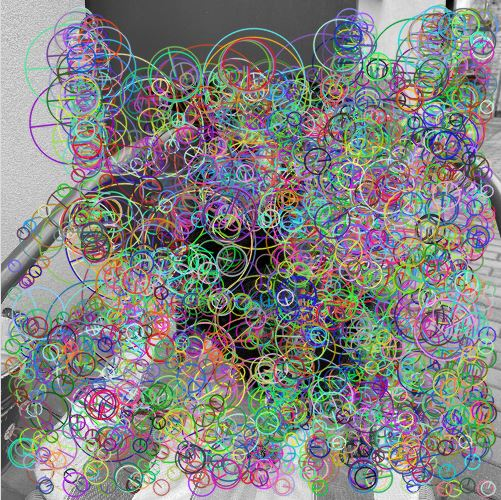
\includegraphics[width=0.50\textwidth]{Figures/surf/surf_example.jpg}
    \caption[SURF key-points and their orientation from an image of a dog]{SURF key-points and their orientation from an image of a dog.}
    \label{fig:surf_example}
\end{figure}

The descriptor is constructed from a square window the size of $20s$ around a key-point. The window is subsequently rotated along with the key-point orientation. Afterwards, this window is divided into $16$ ($4\times4$) square sub-windows. In each sub-window, the features are calculated using $5\times5$ regularly spaced sample points. From these sample points, we calculate the Haar wavelet responses in the horizontal and the vertical direction, where \say{horizontal} and \say{vertical} are defined in relation to the key-point orientation. The responses are weighted with a Gaussian ($\sigma = 3.3s$) centered at the key-point.

Let us call the horizontal responses $d_x$ and the vertical responses $d_y$. Over each sub-window, we denote the sum of the responses $\sum d_x$ and $\sum d_y$, and the sum of absolute values of the responses $\sum |d_x|$ and $\sum |d_y|$. The behavior of these values for different image patterns can be seen in \figref{fig:surf_descriptor}. Combining $\sum d_x$, $\sum d_y$, $\sum |d_x|$, and $\sum |d_y|$ for each of the $16$ sub-window into a vector, we get a descriptor of length $64$.

\begin{figure}
    \centering
    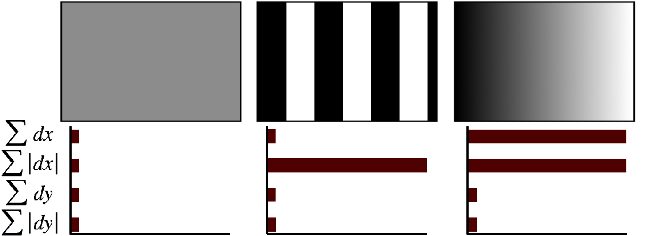
\includegraphics[width=0.8\textwidth]{Figures/surf/surf_descriptor.png}
    \caption[Behaviour of SURF descriptor for different image patterns]{Behaviour of SURF descriptor for different image patterns \cite{Bay2006}.}
    \label{fig:surf_descriptor}
\end{figure}


\section{ORB}
ORB (Oriented FAST and Rotated BRIEF) is a local feature extractor proposed by Ethan Rublee, Vincent Rabaud, Kurt Konolige and Gary Bradski in 2011 \cite{Rublee2011}.

The algorithm builds on a FAST (Features from Accelerated Segment Test) corner detector\cite{Rosten2006} and a BRIEF (Binary Robust Independent Elementary Features) descriptor\cite{Calonder2010}.

\subsection{Key-point Detection}
The ORB algorithm uses FAST-9 variant of the FAST corner detector. This detector compares each pixel intensity (denoted as $I_p$) in an image with the intensities of pixels in circle of radius $9$ around the pixel.

Let $n\in\mathbb{N}$ and threshold $t\in\mathbb{R}^{+}$ be given. Let $S$ be a set of pixels in a circle of radius $9$ around the examined pixel. Let us denote $I_x$ as the intensity of a pixel $x$. The examined pixel is selected as a corner, if there exists a set of $n$ contiguous pixels $S_n \in S$, where $\forall x \in S_n: I_x + t < I_p$, or $\forall x \in S_n: I_x - t > I_p$.

The selected corners, i.e. key-points are then ordered according to a Harris corner measure\cite{Harris1988}. For $N$ key-points, the threshold is selected low enough to get more than $N$ key-points, then the best $N$ key-points (according to Harris corner measure) are selected.

To find multi-scale features, the scale pyramid of an image is generated and key-points are generated at each level in the pyramid.

\subsection{Key-point Description}
To ensure the descriptor's invariance to rotation, we need to determine the key-point orientation. For this, the intensity centroid\cite{Rosin1999} is used. The intensity centroid expects the intensity of a key-point to be offset from its center. The vector from the center to the centroid is used for the key-point orientation.

Given an image $I(x,y)$, the centroid is found using a moment of a patch
\begin{equation}
    m_{pq}=\sum_{x,y} x^p y^q I(x,y).
\end{equation}
The centroid is then located as
\begin{equation}
    C =
    \begin{pmatrix}
        \frac{m_{10}}{m_{00}} \text{, } \frac{m_{01}}{m_{00}}
    \end{pmatrix},
\end{equation}
from which we can obtain the key-point orientation
\begin{equation}
    \theta = \text{atan}2(m_{01},m_{10}),
\end{equation}
where atan$2$ is the quadrant-aware version of arctan.

As an ORB descriptor, a variation on BRIEF descriptor is used. The BRIEF descriptor is a vector of binary values. This allows for fast matching using a Hamming distance.

The descriptor values is computed by comparing random pairs of pixel intensities in a patch. The binary vector is created from the responses on a patch $\boldsymbol{p}$ of test
\begin{equation}
    \tau(\boldsymbol{p};x,y)=
    \begin{cases*}
        1 & if $\boldsymbol{p}(x) < \boldsymbol{p}(y)$ \\
        0 & otherwise
    \end{cases*}, 
\end{equation}
where $\boldsymbol{p}(x)$ is the pixel intensity of a patch $\boldsymbol{p}$ at a point $x$, $x$ and $y$. The pairs of points $x$ and $y$ are from a random predetermined set
\begin{equation}
    \boldsymbol{S} =
    \begin{pmatrix}
        x_1 \dots x_n \\
        y_1 \dots y_n
    \end{pmatrix} 
\end{equation}
where $n$ is the size of our descriptor. The BRIEF descriptor is then defined as a vector of $n$ binary tests:
\begin{equation}
    f_n(\boldsymbol{p}) \coloneqq \sum_{i=1}^{n} 2^{i-1}\tau(\boldsymbol{p};x_i, y_i)
\end{equation}

The steered version of a BRIEF descriptor, according to the orientation $\theta$ of the key-point, can be created by using a corresponding rotation matrix $\boldsymbol{R}_\theta$:
\begin{equation}
    \boldsymbol{S_\theta} = \boldsymbol{R}_\theta \boldsymbol{S}.
\end{equation}
The sets of pairs are precomputed in a lookup table for discretized $\theta$ in increments of $\frac{2\pi}{30}$ to improve speed. In the end, the steered BRIEF descriptor becomes
\begin{equation}
    g_n(\boldsymbol{p}, \theta) \coloneqq f_n(\boldsymbol{p}) | (x_i, y_i) \in \boldsymbol{S}_\theta.
\end{equation}


\section{Bag of Visual Words}
Local feature extractors provide us with varied number of descriptors for each image. However, for classification, we require each image to be represented by a single vector. This can be achieved using a Bag of Words technique.

Bag of Words (BoW) is a technique, which represents each sample in a dataset as a multiset of its words. In general, these words do not have to be literal words but can be any categorization of information provided by the sample.

The first step of BoW is the dictionary generation. The dictionary is a set of $k \in \mathbb{N}$ categories of words called bins. Providing the dictionary, the BoW assigns each word to a bin. Finally, for each sample in the dataset, a histogram of frequencies of words belonging to each bin is calculated.

As an example, we explain the technique with text documents. With text documents, the dictionary consists of every unique word in all documents. The words of each document are assigned to a bin consisting of said words.

For example, in a dictionary consisting of bins [ \say{Peter}, \say{run}, \say{talked}, \say{to} ], a sample sentence \say{Peter talked to Peter} would produce the following histogram:
\begin{equation}
    [2, 0, 1, 1].
\end{equation}

In our case, we consider the descriptors found in an image as words. Since we are dealing with visual information, let us call these words \say{visual words} and designate the BoW technique \say{Bag of Visual Words} (BoVW).

We generate the categories using a $k$-means algorithm on all the visual words in the training dataset. Afterwards, we assign the visual words to the closest (considering euclidean distance) category and compute the histogram of frequencies.

\subsection{$k$-means}
The $k$-means algorithm is an unsupervised learning technique \cite{macqueen1967}. Let $X=\{ x_1, x_2, \dots, x_n \}$ be a dataset of $n$ data-points. The goal is to assign the data points into $k$ clusters $S = \{ S_1, S_2, \dots, S_k \}$, such that
\begin{equation}
    \argmin_S \sum_{i=1}^k \sum_{x\in S_i} \norm{x-c_i}^2,
\end{equation}
where \(c_1, c_2, ..., c_k \) are the centroids of corresponding clusters \(S_1, S_2, ..., S_k \). The centroids are determined as means of data points belonging to each cluster.

The algorithm starts by selecting $k$ random data points as the centroids. The iterative process is based on the alternation between the following two consecutive steps until a termination condition is met:
\begin{description}
    \item{\textbf{Assignment step:}} Each data point is assigned to the cluster, such that the Euclidean distance between the centroids of the clusters and the data point is the smallest one.
    \item{\textbf{Update step:}} For each cluster, a new centroid is computed as the mean value of data points belonging to this cluster.
\end{description}

The termination condition is satisfied, when the ratio of the samples, for which the assigned cluster changes, to the total amount of samples, is smaller than a specified threshold. The steps of the algorithm are demonstrated in \figref{fig:k_means_alg}.
\begin{figure}[ht]
    \centering
    \begin{subfigure}[t]{0.22\textwidth}
        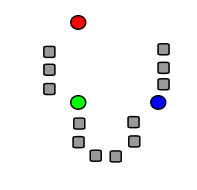
\includegraphics[width=\textwidth]{Figures/k-means/k-means_inicial_step.png}
        \caption{At first, random data points are selected as the initial $k$ centroids.}
        \label{fig:k-means-alg:inicial_step}
    \end{subfigure}\hfill
    \begin{subfigure}[t]{0.22\textwidth}
        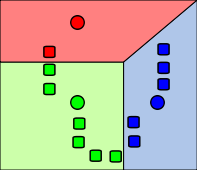
\includegraphics[width=\textwidth]{Figures/k-means/k-means_assignment_step.png}
        \caption{By choosing the nearest centroid, each data point is assigned to a corresponding cluster.}
        \label{fig:k-means-alg:assignment_step}
    \end{subfigure}\hfill
    \begin{subfigure}[t]{0.22\textwidth}
        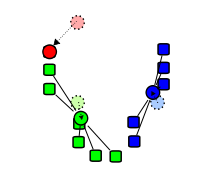
\includegraphics[width=\textwidth]{Figures/k-means/k-means_update_step.png}
        \caption{New centroids are calculated as mean values of data points in the cluster.}
        \label{fig:k-means-alg:update_step}
    \end{subfigure}\hfill
    \begin{subfigure}[t]{0.22\textwidth}
        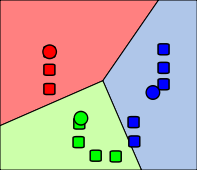
\includegraphics[width=\textwidth]{Figures/k-means/k-means_assignment_step_2.png}
        \caption{Steps in (b) and (c) are repeated until the terminate condition is met.}
        \label{fig:k-means-alg:assignment_step_2}
    \end{subfigure}\hfill
    \caption[Lloyd's algorithm demonstration.]{Lloyd algorithm demonstration \cite{Wikikmeans}.}
    \label{fig:k_means_alg}
\end{figure}
The challenge is the determination of the number of clusters $k$, the size of the visual dictionary. In our experiments, we examine different settings for $k$ to find a clustering, which allows for satisfactory classification.


\section{PCA}
PCA (Principal Component Analysis) is a global feature extractor. It is used to reduce the dimension of data while preserving as much of the data variance as possible.

Let $x_t \in \mathbb{R}^n$ be a data point, where $t=1,\dots,T$ and $T$ is the amount of data points. We want to project $x_t$ into a $y_t \in \mathbb{R}^k$, where $k < n$. We want to find the optimal parameters $P$ of the parametric reduction mapping $\psi_P: \mathbb{R}^n \rightarrow \mathbb{R}^k$ and the parametric reconstruction mapping $\psi_P^{-1}: \mathbb{R}^k \rightarrow \mathbb{R}^n$. The optimal parameters $P^{*}$ minimize the reconstruction error, i.e.,
\begin{equation}
    P^{*} \coloneqq \argmin_{P \in \rho} \sum_{t=1}^T \norm{x_t - \psi_P^{-1}(\psi_P(x_t))},
    \label{eq:mapping_optimization}
\end{equation}
where $\psi$ denotes the set of feasible parameters and $\norm{x_t - \psi_P^{-1}(\psi_P(x_t))}$ is the reconstruction error of a datapoint.

PCA uses the mappings
\begin{equation}
    \psi_{[Q,b]}^{-1}(y) \coloneqq Qy+b, \psi_{[Q,b]}(x) \coloneqq Q^{\top}(x-b),
    \label{eq:pca_mappings}
\end{equation}
with parameters $b \in \mathbb{R}^n$ and $Q \in \mathbb{R}^{n,k}$ with orthonormal columns, i.e.,
\begin{equation}
    Q^{\top}Q = I \in \mathbb{R}^{k,k}.
    \label{eq:pca_identity}
\end{equation}

Substituing \eqref{eq:pca_mappings}, \eqref{eq:pca_identity} into the optimization problem \eqref{eq:mapping_optimization} and using the square Euclidean norm for meassuring the reconstruction error, we get the optimization problem
\begin{equation}
    [Q^{*}, b^{*}] \coloneqq \argmin_{Q,b} \sum_{t=1}^T \norm{x_t - (QQ^{\top}(x_t-b) + b)}^2_2 \text{s.t.} Q^{\top}Q=I.
    \label{eq:pca_optimization}
\end{equation}
The objective function $f(Q,b)$ of \eqref{eq:pca_optimization} can be rewritten to the form
\begin{equation}
    f(Q,b)=\sum_{t=1}^T (x_t^{\top}x_t - 2 x_t^{\top}b + b^{\top}b - x_t^{\top}QQ^{\top}x_t + 2x_t^{\top}QQ^{\top}b - b^{\top}QQ^{\top}b),
    \label{eq:pca_obj_fun}
\end{equation}
and the optimality condition of $b^{*}$ can be formulated as
\begin{equation}
    \nabla_bf(Q,b) = \sum_{t=1}^T(-2x_t+2b+2QQ^{\top}xt-2QQ^{\top}b)=0,
\end{equation}
which is equivalent to
\begin{equation}
    (I-QQ^{\top})\sum_{t=1}^T(b-x_t)=0.
    \label{eq:pca_opt_b}
\end{equation}
As $k<n$, $Q \in \mathbb{R}^{n,k}$ is not a full column rank and $QQ^{\top} \neq = I$. The unique solution of \eqref{eq:pca_opt_b} is
\begin{equation}
    b^{*} = \frac{1}{T}\sum_{t=1}^T x_t.
\end{equation}
Moreover, the Hessian matrix
\begin{equation}
    \nabla_{b,b}^2 f(Q,b)=2(I-QQ^{\top}),
    \label{eq:pca_sol_b}
\end{equation}
is symmetric positive definitive matrix, therefore the objective function \eqref{eq:pca_obj_fun} is strictly convex (in the variable $b$) and \eqref{eq:pca_sol_b} is unique minimizer.

Let us denote the shifted data by
\begin{equation}
    \hat{x_t} \coloneqq x_t - b^* , t=1, \dots, T
\end{equation}
and write the objective function of \eqref{eq:pca_obj_fun} as
\begin{equation}
    f(Q,b^*) = \sum_{t=1}^T \norm{\hat{x_t} - QQ^{\top}\hat{x_t}}_2^2 = \sum_{t=1}^T (\hat{x_t}^{\top}\hat{x_t} - \hat{x_t}^{\top} QQ^{\top} \hat{x_t}).
    \label{eq:pca_obj_fun_Q}
\end{equation}
We can simplify \eqref{eq:pca_obj_fun_Q} using properties of the matrix trace:
\begin{equation}
    f(Q,b^*) = \sum_{t=1}^T \text{trace} (\hat{x_t}^{\top}\hat{x_t}) - \sum_{t=1}^T \text{trace} (\hat{x_t}^{\top} QQ^{\top} \hat{x_t})
    = \text{trace}(\text{cov}(x)) - \text{trace}(Q^{\top} \text{cov}(x) Q ),
\end{equation}
where cov($x$) is the covariance matrix of $x$ defined as
\begin{equation}
    \text{cov}(x) \coloneqq \sum_{t=1}^T(x_t-b^*)(x_t-b^*)^{\top} = \sum_{t=1}^T\hat{x_t}\hat{x_t}^{\top}.
\end{equation}
The argument of the minimum is independent of constants in the objective function. Therefore, we can reformulate the optimization problem \eqref{eq:pca_optimization} (in terms of variable $Q$) as
\begin{equation}
    \begin{split}
        [Q^*] &= \argmin_{Q^{\top}Q=I} f(Q,b^*) = \argmin_{Q^{\top}Q=I} -\text{trace}(Q^{\top}\text{cov}(x)Q) \\&= \argmax_{Q^{\top}Q=I} \text{trace}(Q^{\top}\text{cov}(x)Q) \\&= \argmax_{\forall j:q_j^{\top}q_j=1} \sum_{j=1}^k q_j^{\top} \text{cov}(x) q_j,
    \end{split}
    \label{eq:pca_optimization_final}
\end{equation}
where $q_j , j=1,\dots,k$ denote the (orthonormal) columns of the matrix $Q \in \mathbb{R}^{n,k}$. The Lagrange function corresponding to the problem \eqref{eq:pca_optimization_final} is given by
\begin{equation}
    L(Q, \lambda) \coloneqq \sum_{j=1}^k q_j^{\top} \text{cov}(x)q_j - \sum_{j=1}^k \lambda_j (q_j^{\top} q_j - 1),
\end{equation}
where $\lambda \in \mathbb{R}^K$ denotes Lagrange multiplier correponding to equality constraints. The first Karush-Kuhn-Tucker conditions can be derived as
\begin{equation}
    \nabla_{q_j}L(Q,\lambda) = 2 \text{cov}(x)q_j-2\lambda_jq_j=0, j=1,\dots,k,
\end{equation}
which are the eigenvalue equations
\begin{equation}
    \text{cov}(x)q_j=\lambda_j q_j, j=1,\dots,k.
    \label{eq:pca_eig}
\end{equation}
If we substitute \eqref{eq:pca_eig} into objective function \eqref{eq:pca_optimization_final}, we get
\begin{equation}
    \sum_{j=1}^k q_j^{\top} \text{cov}(x)q_j = \sum_{j=1}^k \lambda_j q_j^{\top}q_j = \sum_{j=1}^k \lambda_j.
\end{equation}
As the problem \eqref{eq:pca_optimization_final} is maximization problem, the optimal $Q^*$ consists of (orthonormal) eigenvectors which correspond to $k$ largest eigenvalues.


